% Horizon penetrating coordinates (vs. Schwarzschild coordinates)
% for a black hole spacetime, with excision
% Author: Jonah Miller
\documentclass[tikz,border=6pt]{standalone}
\usepackage{tikz}
\usetikzlibrary{arrows}
\usetikzlibrary{arrows.meta}
\usetikzlibrary{decorations.markings}
\usepackage{pgfplots}

%\tikzset{>={Latex[length=3mm]}}

\begin{document}
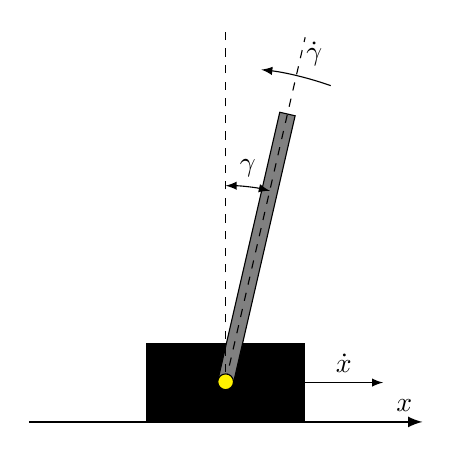
\begin{tikzpicture}[>= latex]

\def\polelength{3}
\def\angle{-13}
\def\poleheight{1}
\def\radiusone{2.5}
\def\radiustwo{4}

%\draw[-,thick] (-3,0) -- (3,0);
\draw[-,fill=black] (-1,0) rectangle(1,\poleheight) {};



\draw[-,fill=gray,rotate around={\angle:(0,{0.5\poleheight})}] (-0.1,{0.5\poleheight}) rectangle(0.1,{\poleheight + \polelength}) {};
\draw[-,dashed,rotate around={\angle:(0,{0.5\poleheight})}] (0,{0.5\poleheight}) -- (0,{\polelength + \poleheight + 1});


\draw[-,dashed] (0,0) -- (0,{\polelength+\poleheight+1});
\draw[-,fill=yellow] (0,{0.5\poleheight}) circle(0.1);

%\draw[->] ({3*sin(13)},{\poleheight/2 + 3*cos(\angle)}) -- (0,{3+\poleheight/2});
\draw[<->] ({\radiusone*sin(-\angle)},{\poleheight/2 + \radiusone*cos(\angle)}) arc ({90+\angle}:90:{\radiusone}) node[midway, above]{$\gamma$};

%\draw[<-] ({\radiustwo*sin(-\angle)},{\poleheight/2 + \radiustwo*cos(\angle)}) arc ({90+\angle}:90:{\radiustwo}) node[midway, above]{$\dot{\theta}$};


\draw[<-] ({\radiustwo*sin(-\angle-6.5)},{\poleheight/2 + \radiustwo*cos(\angle+6.5)}) arc ({90+\angle+6.5}:{90+\angle-6.5}:{\radiustwo}) node[midway, above right]{$\dot{\gamma}$};



\draw[->] (1,{\poleheight/2}) -- (2,{\poleheight/2}) node[midway,above]{$\dot{x}$};

\draw[->, thick] (-2.5,0) -- (2.5,0) node[above left]{$x$};

\end{tikzpicture}
\end{document}